\documentclass[10pt, border=3mm]{standalone}
%\usepackage{pstricks-add}
\usepackage{tikz}
\usetikzlibrary{positioning, calc, graphs}

\definecolor{vq_grey}{RGB}{225,225,219}
\pagecolor{vq_grey}

\begin{document}

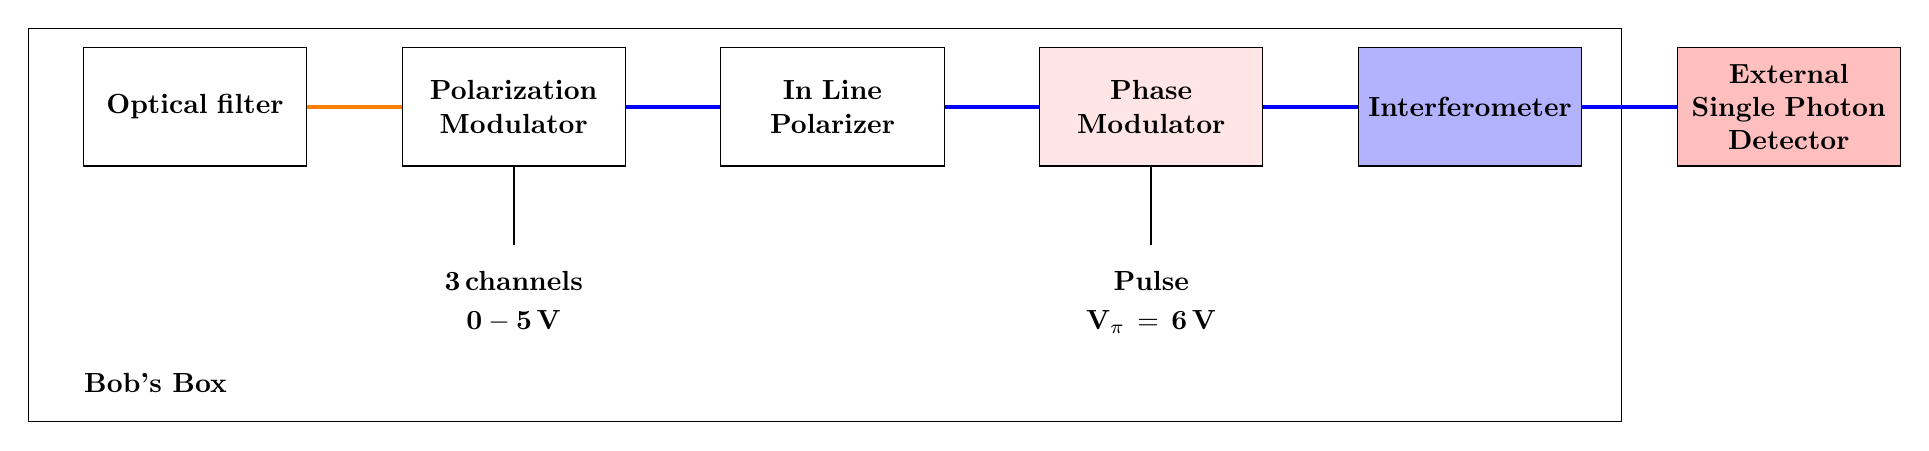
\begin{tikzpicture}[block/.style={rectangle,draw,minimum height=1.5cm,text width=2.6cm,align=center},node distance = 12mm , block2/.style={-, rectangle,draw,minimum height=5cm,text width=20cm,align=center}  ]
\node (b1) [block, fill=white] {\textbf{Optical filter}} ;
\node (b2) [block, right=of b1, fill=white] {\textbf{Polarization Modulator}};
\node (b3) [block,right=of b2, fill=white] {\textbf{In Line Polarizer}};
\node (b4) [block, fill=pink!40,right=of b3] {\textbf{Phase Modulator}} ;
\node (b5) [block, fill=blue!30, right=of b4] {\textbf{Interferometer}} ;
\node (b6) [block,right=of b5, fill=pink] {\textbf{External Single Photon Detector}} ;
\node (b15) [block2] at (8,-1.5) {};
  \begin{scope}
    \draw [-, orange, very thick] (b1) -- (b2);
    \draw [-, blue, very thick] (b2) -- (b3);
    \draw [-, blue, very thick] (b3) -- (b4);
    \draw [-, blue, very thick] (b4) -- (b5);
    \draw [-, blue, very thick] (b5) -- (b6);
    \draw [-, black, thick] ($(b2.south)+(0,0)$) -- ($(b2.south)+(0,-1)$);
    \node (input) [below  = 1.2cm and -2cm of  b2, name=f]{$\mathbf{3 \, channels}$};
    \node (input) [below  = 1.7cm and -2cm of  b2, name=f]{$\mathbf{ 0 - 5  \,V}$};
    \draw [-, black, thick] ($(b4.south)+(0,0)$) -- ($(b4.south)+(0,-1)$);
    \node (input) [below  = 1.2cm and -2cm of  b4, name=f]{$\mathbf{Pulse}$};
    \node (input) [below  = 1.7cm and -2cm of  b4, name=f]{$\mathbf{ V _\pi \,= \,6 \,V}$};
    \node (input) at (-0.5,-3.5){\textbf{Bob's Box}};
  \end{scope}
\end{tikzpicture}
\end{document}
